\chapter{Specifiche dell'applicazione}
\label{chapter1}
In questo capitolo verrà analizzata la parte delle specifiche dell'applicazione, ovvero tutto ciò che è stato fatto prima dello sviluppo del progetto e dell'implementazione dell'app.
\\Quindi, che cos'è la Walkability, il target di utenza a cui si è deciso rivolgersi, gli obiettivi principali dell'app ed il Material Design.


\section{Walkability}
Come già accennato all'interno dell'introduzione, il termine walkability, generalmente, indica il livello di comfort e sicurezza per i pedoni in una certa area urbana.
\\La walkability ha benefici per la salute, l'ambiente e l'economia. 
\\I fattori che influenzano maggiormente una buona walkability sono: presenza o assenza di marciapiedi, la qualità di essi, condizioni del traffico e delle condizioni stradali, accessibilità e sicurezza degli edifici, sicurezza generale dell'area urbana interessata.
\\La walkability è un concetto importante nella progettazione urbana sostenibile \cite{walkability}.
\\Attualmente si parla molto di creare ambienti percorribili e di migliorare la walkabilty.
\\Tali strategie sono pensate per risolvere numerosi problemi derivanti dalla mancanza di vitalità del centro città come la congestione del traffico, l'ingiustizia ambientale e l'isolamento sociale \cite{walkable}.
\\Allo stato attuale, esistono due trend in continua crescita: uno è quello dell’invecchiamento della popolazione e l’altro è quello dell’urbanizzazione.
\\Proprio per questo si è cominciato a pensare come dovrebbe essere strutturata una città del futuro e si è così cominciato a parlare di walkability.
\\Si può osservare la figura \ref{fig:invecchiamento}, che raffigura l'invecchiamento delle persone negli ultimi, e futuri, 30 anni:
\pagebreak
\begin{figure}[!h]
    \centering
	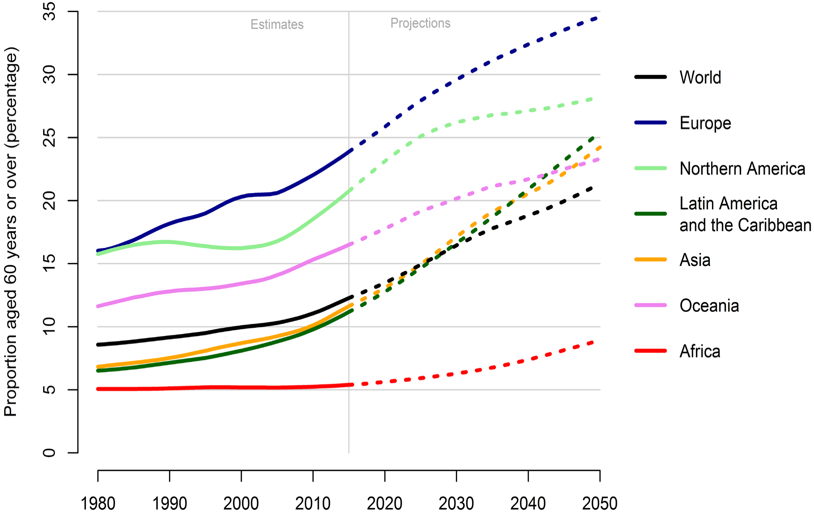
\includegraphics{Tesi/images/invecchiamento-popolazione.png}
	\caption{\textit{Invecchiamento popolazione \cite{invecchiamento}}}
	\label{fig:invecchiamento}
\end{figure}
\\Invece si può osservare, la figura \ref{fig:urbanizzazione}, che raffigura l'andamento dell'urbanizzazione globale negli anni passati, ed una previsione nei prossimi:
\begin{figure}[!h]
    \centering
	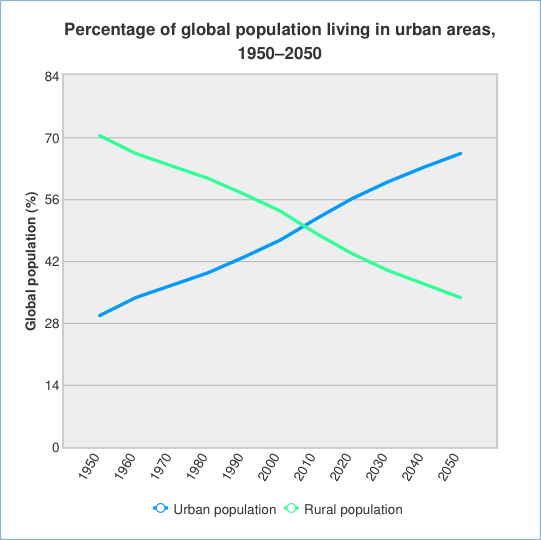
\includegraphics{Tesi/images/urbanizzazione.png}
	\caption{\textit{Urbanizzazione \cite{urbanizzazione}}}
	\label{fig:urbanizzazione}
\end{figure}
\pagebreak
\subsection{Punti chiave della Walkability}
I punti principali, per cui una città abbia una buona walkability, sono i seguenti:
\begin{itemize}
    \item \textbf{Ambienti attraversabili}: hanno le condizioni fisiche di base per consentire alle persone di spostarsi da un luogo all'altro senza grandi impedimenti, ad esempio percorsi relativamente regolari.
    \item \textbf{Luoghi compatti}: forniscono brevi distanze alle destinazioni per coloro che camminano per utilità.
    \item \textbf{Sicurezza}: è fondamentale in quanto, ad esempio, il crimine percepito e la sicurezza del traffico percepita riguardano un potenziale danno per la persona.
    \item \textbf{Ambienti fisicamente attraenti}: presenza di strutture pedonali come marciapiedi o percorsi, attraversamenti pedonali contrassegnati, illuminazione appropriata e arredo urbano, segnaletica utile e alberi da strada. 
    \\Possono anche includere un'architettura interessante, viste piacevoli e servizi, che permettono alle persone di muoversi liberamente senza l'utilizzo delle automobili.
\end{itemize}
Di solito, un \textit{\textbf{walkable environment}}, ovvero un ambiente con una buona walkability, è definito tale, quando è vivace, socievole, piacevole, pulito e pieno di persone interessanti.
\cite{walkable}.

\section{Target utenti}

Il target di utenza, a cui si è deciso rivolgersi, sono utenti anziani, o comunque tutti quegli utenti che si muovono in un'area urbana ristretta, vicina alla propria abitazione.
\\L'applicazione, in ogni caso, potrà essere utilizzata anche da qualsiasi altro utente che avrà piacere di condividere foto, video, note vocali o note scritte inerenti all'area urbana interessata. Sia per quanto riguarda esperienze positive, che negative.
\\Optare per questo tipo di utenza, ha fatto si, di adottare, alcune scelte implementative, rispetto ad altre, che verranno definite nel capitolo \ref{chapter2}.
\\Inoltre, aver scelto questo tipo di utenza, ha fatto in modo di scegliere, a maggior ragione, il sistema operativo Android, in quanto più diffuso.


\section{Obiettivi}

Gli obiettivi principali del progetto (e quindi dell'applicazione) sono:
\begin{itemize}
\item Visualizzare la posizione corrente dell'utente all'interno di una mappa GPS servita da Google Maps
\item Permettere all'utente di creare una nota caratterizzata da elementi multimediali
\item Permettere all'utente di inserire nella nota: foto, video, note vocali, una nota scritta, nome del luogo ed indirizzo in cui si trova
\item Visualizzare e permettere all'utente di scegliere se eliminare alcuni, o tutti, gli elementi acquisiti fino a quel momento
\item Visualizzare il numero di elementi multimediali acquisiti fino a quel momento
\item Inviare il contenuto della nota al repository centralizzato
\end{itemize}

\section{Interfaccia utente}
In questa sezione verrà presentato il Material Design.
\\Un requisito fondamentale dell'applicazione, è stato renderla il più intuitiva e semplice possibile da utilizzare, visto il target utenza scelto.
\\Dunque l'interfaccia è stata pensata ed ideata secondo le linee guida del Material Design, che verrà presentato ed introdotto nella sezione \ref{materialdesign}.
\\Successivamente nella sezione \ref{design} verranno presentati gli elementi utilizzati di Material Design.

\subsection{Material Design}
\label{materialdesign}
Il Material Design è un design sviluppato da Google, annunciato il 25 giugno 2014 in occasione del Google I/O.
\\Il Material Design è supportato nativamente a partire da Android 5.0, ma può essere utilizzato nelle versioni precedenti attraverso la libreria v7 appcompat disponibile agli sviluppatori. 
\\Per questa applicazione, si è fatto fede, ad alcune linee guida del Material Design.
\\\\Il Material Design è un linguaggio visuale che sintetizza i principi classici del buon design con l'innovazione della tecnologia e della scienza, ovvero, sviluppa un singolo sistema sottostante che unifica l'esperienza utente su piattaforme, dispositivi e metodi di input.
\\Sviluppa un singolo sistema sottostante che unifica l'esperienza utente su piattaforme, dispositivi e metodi di input.
\\Il Material Design è ispirato al mondo fisico, compreso il modo in cui riflettono la luce e si proiettano le ombre.
\\Il Material Design è guidato da metodi di progettazione della stampa (tipografia, griglie, spazio, scala, colore e immagini) per creare una gerarchia, significato e concentrazione per immergere gli spettatori nell'esperienza.
\\Il Material Design, focalizza l'attenzione e mantiene la continuità, attraverso sottili feedback e transizioni coerenti. Quando gli elementi appaiono sullo schermo, trasformano e riorganizzano l'ambiente, con interazioni che generano nuove trasformazioni.
\\Il Material Design mantiene la stessa interfaccia utente su tutte le piattaforme, utilizzando componenti condivisi su Android, iOS, Flutter e sul web \cite{materialdesign}.